\documentclass[11pt,a4paper]{article}
\usepackage[margin=2.5cm]{geometry}
\usepackage{graphicx}
\usepackage{booktabs}
\usepackage{amsmath}
\usepackage[hyphens]{url}
\usepackage{hyperref}
\usepackage{xcolor}
\usepackage{caption}
\usepackage{subcaption}
\usepackage{float}
\usepackage{microtype}
\emergencystretch=2em

\title{Experimental Notes for Rebuttal\\[0.3em]
\large Scaling up Measurement-Noise Scaling Laws}
\author{}
\date{June 2026}

\begin{document}
\maketitle
\tableofcontents
\clearpage

%% ============================================================
\section{Finding the Data}

All code, data pointers, and results described in this document live in the
following repository:

\begin{center}
\url{https://github.com/igor-sadalski/Scaling-up-measurement-noise-scaling-laws.git}
\end{center}

\noindent The experiments described here were run on the \textbf{\texttt{adding-state}}
branch.
Raw data and trained model checkpoints are not stored in the repository itself;
they live on S3 at \path{s3://measurement-noise-scaling-laws/data/} and can
be accessed locally via the \texttt{S3Retriever} utility in
\path{scaling_laws/s3_retriever.py}.
The local data root defaults to \path{~/noise_scaling/data/}
and can be overridden with the \texttt{NOISE\_SCALING\_DATA\_DIR} environment
variable.
All result CSV and PNG files referenced throughout this document are committed
to the repository under \path{analysis/final_results/}.
\clearpage

%% ============================================================
\section{Geneformer Validation Loss Scaling}

Geneformer was implemented as a BERT-style masked-language model
(\texttt{BertForMaskedLM}) using the HuggingFace Trainer.
The control architecture used throughout has 256 hidden dimensions,
4 attention heads, 3 transformer layers, a 512-dimensional feedforward
(intermediate) layer, maximum input length of 512 tokens, and attention
and hidden dropout of 0.02.
Training used a masked-language-modelling objective with 15\% token masking,
AdamW optimiser, learning rate $10^{-3}$, weight decay $0.001$,
5\,000 warmup steps with a linear decay schedule, and a per-device
batch size of 64.
Early stopping monitored validation loss with patience 5;
checkpoints were saved every 1\,000 optimiser steps.
Experiments were run across a $10 \times 10$ grid of cell counts and
quality levels for all four datasets (PBMC, larry, MERFISH, shendure),
yielding 400 experiments per dataset.
After training, the saved best-checkpoint model was loaded and
\texttt{GeneformerPretrainer.evaluate()} was run on the held-out
\textbf{test} split (separate from the validation split used during
training), producing a masked-language-modelling cross-entropy loss
saved to \texttt{test\_loss.txt}.
This is a fresh inference pass on unseen data, not the validation loss
recorded in the training log.
These 400 scalar values were plotted on a log--log scale and a
power law $\mathcal{L}(N) \propto N^{-\alpha}$ was fitted independently
for each quality level using ordinary least squares on the log-transformed
values.

\medskip
\noindent\textbf{Data:} \path{analysis/final_results/geneformer_loss_scaling.csv}

\begin{figure}[H]
\centering
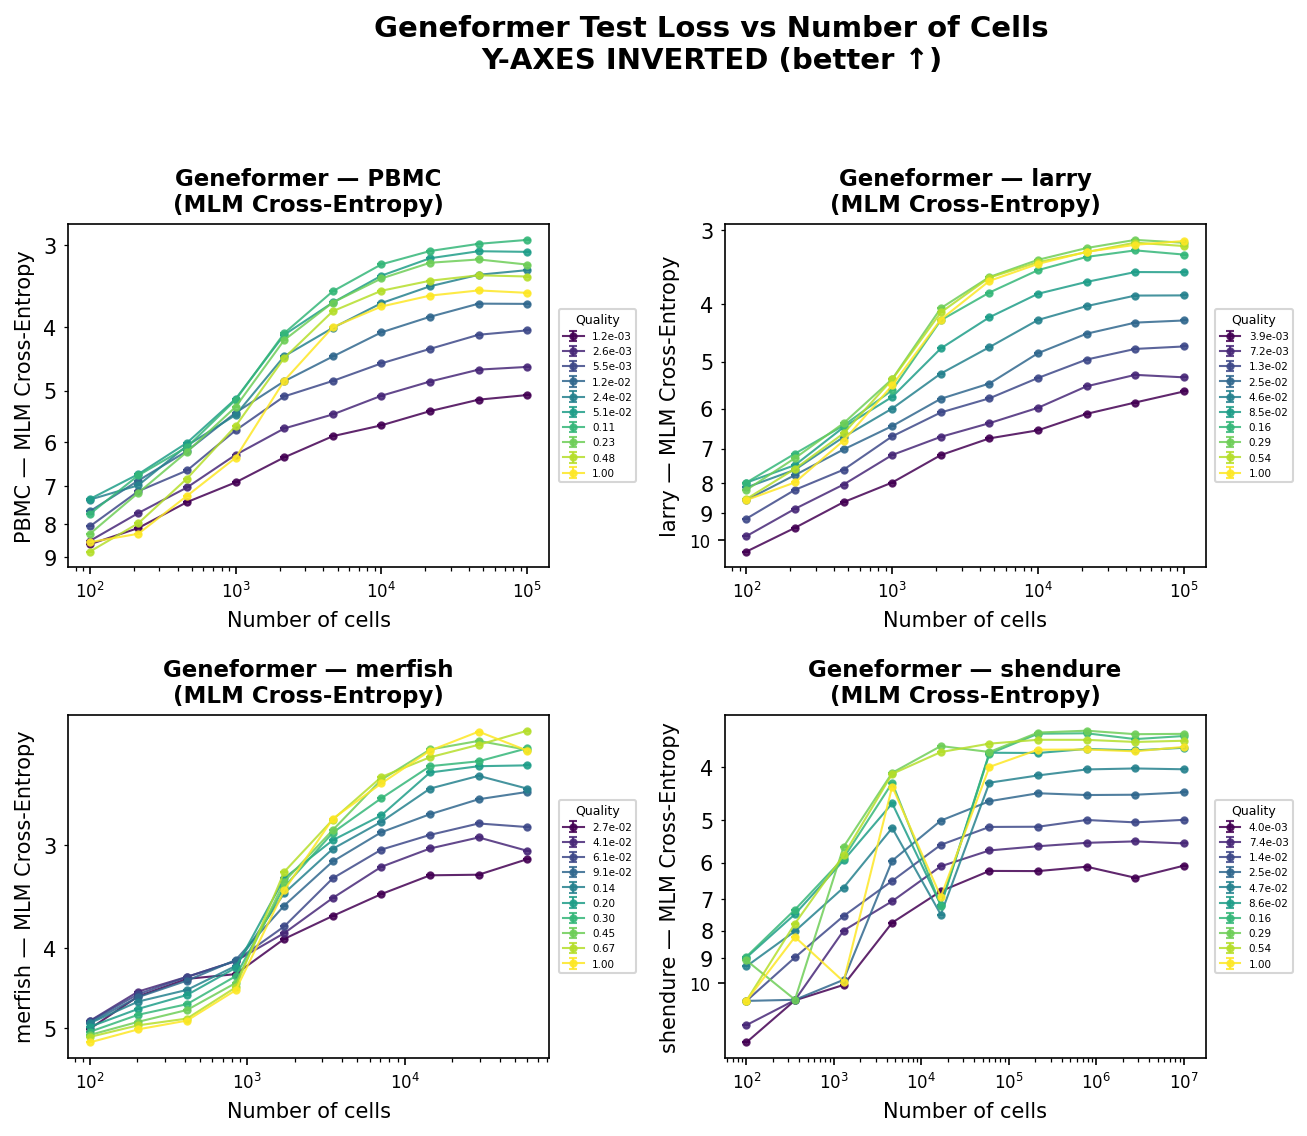
\includegraphics[width=\textwidth,height=0.65\textheight,keepaspectratio]{../final_results/geneformer_loss_scaling.png}
\caption{Geneformer final validation loss vs.\ training-set size on a
log--log scale, with power-law fits per quality level.}
\label{fig:loss_scaling}
\end{figure}
\clearpage

%% ============================================================
\section{Geneformer Training Dynamics}

Training and validation loss trajectories were collected for every
Geneformer experiment using the same architecture and training protocol
described in Section~\ref{fig:loss_scaling}
(256 hidden, 4 heads, 3 layers, 512 FFN, lr $= 10^{-3}$,
batch size 64, early stopping patience 5).
Loss histories were read from the \texttt{log\_history} field of
\texttt{trainer\_state.json}; each entry records the global step,
training loss, and evaluation loss.
To keep the figure readable, each trajectory was subsampled to
50 data points selected by evenly-spaced row index (not by step value),
and the best checkpoint --- identified from the
\texttt{best\_model\_checkpoint} field written by the HuggingFace
Trainer into \texttt{trainer\_state.json} --- was marked with a cross.
Three size ranks --- the smallest, a middle, and the largest available
cell count --- were selected per dataset and plotted together in
a single multi-panel figure.
Early-stopping patience for Geneformer was 3 evaluation rounds
(i.e.\ 3\,000 steps without improvement).

\medskip
\noindent\textbf{Data:} \path{analysis/final_results/geneformer_loss_curves_sml.csv}

\begin{figure}[H]
\centering
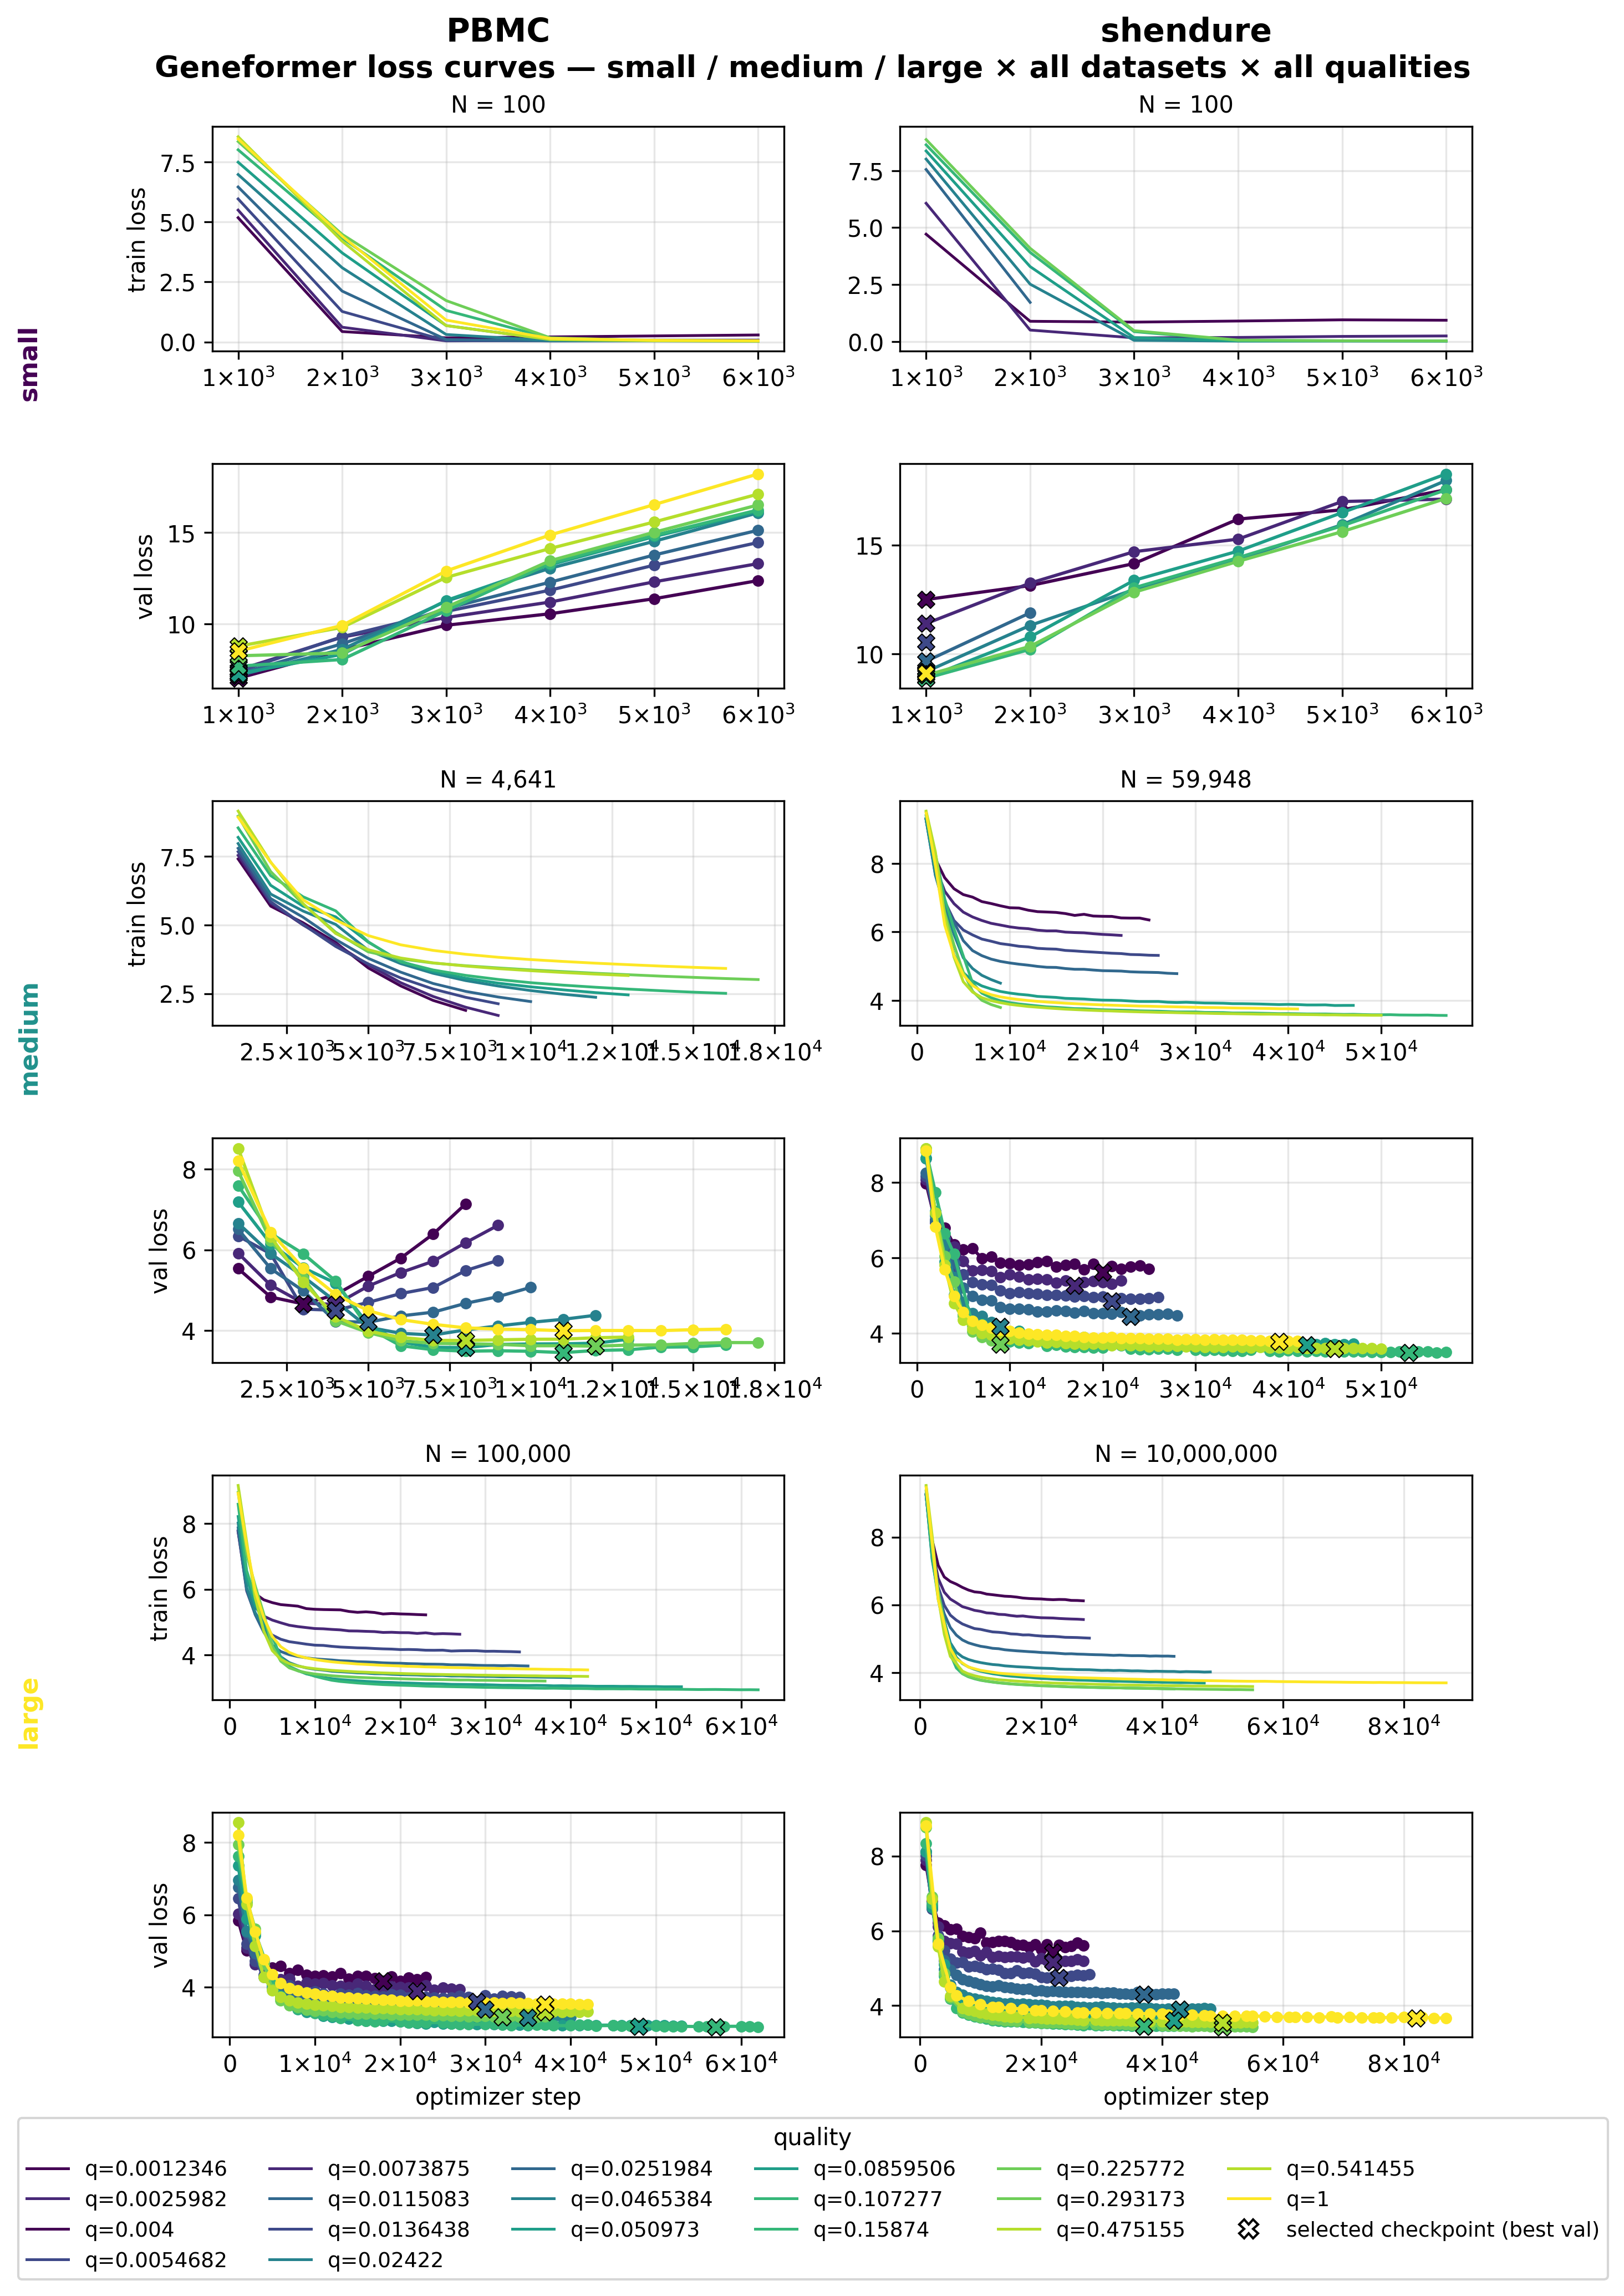
\includegraphics[width=\textwidth,height=0.65\textheight,keepaspectratio]{../final_results/geneformer_loss_curves_sml.png}
\caption{Geneformer training (solid) and validation (dashed) loss curves
for three size ranks across all datasets.
Crosses mark the early-stopping checkpoint.}
\label{fig:loss_curves}
\end{figure}
\clearpage

%% ============================================================
\section{Geneformer Model-Capacity Scaling}

Seven Geneformer configurations were trained on PBMC at the largest
available cell count (100\,000 cells) across all ten quality levels.
The configurations span a range of roughly 0.012M to 56.62M body
parameters by jointly scaling embedding dimension, number of layers,
number of attention heads, and feedforward width:

\begin{table}[H]
\centering
\small
\begin{tabular}{rrrrrr}
\toprule
Embed dim & Layers & Heads & FFN & Max input & Body params (M) \\
\midrule
32  & 1 & 1 &   64 & 512 & $\sim$0.012 \\
64  & 2 & 1 &  128 & 512 & $\sim$0.098 \\
128 & 2 & 2 &  256 & 512 & $\sim$0.39  \\
256 & 3 & 4 &  512 & 512 & $\sim$2.36  \\
384 & 4 & 6 &  768 & 512 & $\sim$7.08  \\
512 & 6 & 8 & 1024 & 512 & $\sim$18.87 \\
768 & 8 &12 & 1536 & 512 & $\sim$56.62 \\
\bottomrule
\end{tabular}
\caption{Geneformer architecture sweep configurations.
The 256-dim row (control) matches the configuration used in
all other experiments.}
\end{table}

All configurations shared the same training hyperparameters:
AdamW, lr $= 10^{-3}$, weight decay $0.001$, 5\,000 warmup steps,
linear schedule, batch size 64, 40\,000 total optimiser steps,
early stopping patience 5 (eval every 1\,000 steps, metric:
\texttt{eval\_loss}).
After training, cell embeddings were extracted with
\texttt{EmbExtractor} and LMI was computed on the
\texttt{protein\_counts} signal.
MI was plotted against total trainable parameter count on a log--log
scale.

\medskip
\noindent\textbf{Data:} \path{analysis/final_results/geneformer_model_size_sweep.csv}

\begin{figure}[H]
\centering
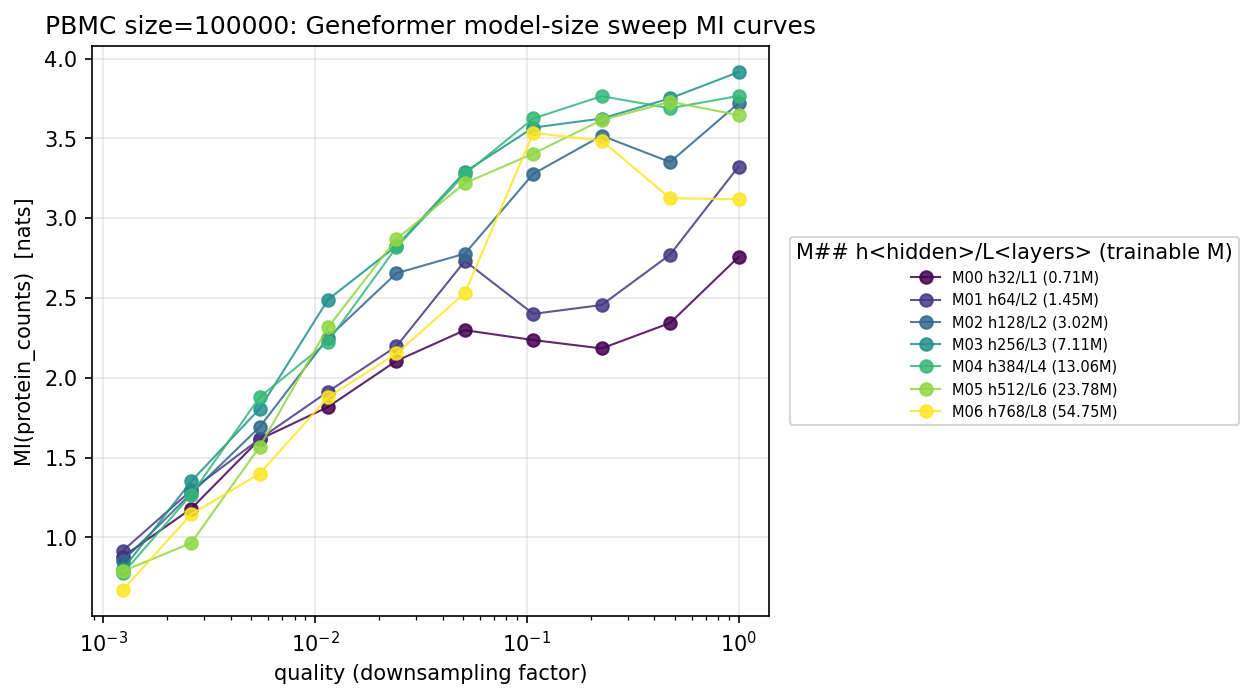
\includegraphics[width=0.85\textwidth,height=0.65\textheight,keepaspectratio]{../final_results/geneformer_model_size_sweep.png}
\caption{Geneformer MI on PBMC \texttt{protein\_counts} signal
vs.\ total trainable parameters for seven architecture configurations,
}
\label{fig:geneformer_model_sweep}
\end{figure}
\clearpage

%% ============================================================
\section{STATE Hyperparameter Sweep}

The STATE model architecture was held fixed throughout:
256-dimensional token embeddings (\texttt{emsize}$=256$),
512-dimensional feedforward layer (\texttt{d\_hid}$=512$),
4 attention heads, 3 transformer layers, and 256-dimensional output
projection (\texttt{output\_dim}$=256$).

A grid search over four hyperparameters was run on PBMC at the
largest cell count (100\,000 cells) across all ten quality levels:

\begin{table}[H]
\centering
\small
\begin{tabular}{ll}
\toprule
Hyperparameter & Values searched \\
\midrule
Dropout & 0.0, 0.1, 0.2, 0.3 \\
Batch size & 32, 64, 128 \\
Peak learning rate & $10^{-6}$, $10^{-5}$, $5\times10^{-5}$, $10^{-4}$, $5\times10^{-4}$, $10^{-3}$ \\
Weight decay & $10^{-4}$, $10^{-3}$, $10^{-2}$, $10^{-1}$ \\
\bottomrule
\end{tabular}
\caption{STATE hyperparameter search space.
Eight random configurations were sampled plus one production config
(dropout 0.1, batch 64, lr $10^{-4}$, wd $10^{-2}$), giving 9 trials.}
\end{table}

Every trial was trained for exactly 15\,000 optimiser steps using AdamW.
Validation loss was checked every 1\,000 steps (limited to 50 batches
per check); early stopping used patience 5.
LMI was computed at the best checkpoint on the \texttt{protein\_counts}
signal.
The figure shows one curve per HP trial: MI on the \texttt{protein\_counts}
signal plotted against quality (log scale) for each of the 9 configurations,
allowing a direct visual comparison of how each set of hyperparameters
affects MI across the full quality range.

\medskip
\noindent\textbf{Data:} \path{analysis/final_results/hyperpam_sweep.csv}

\begin{figure}[H]
\centering
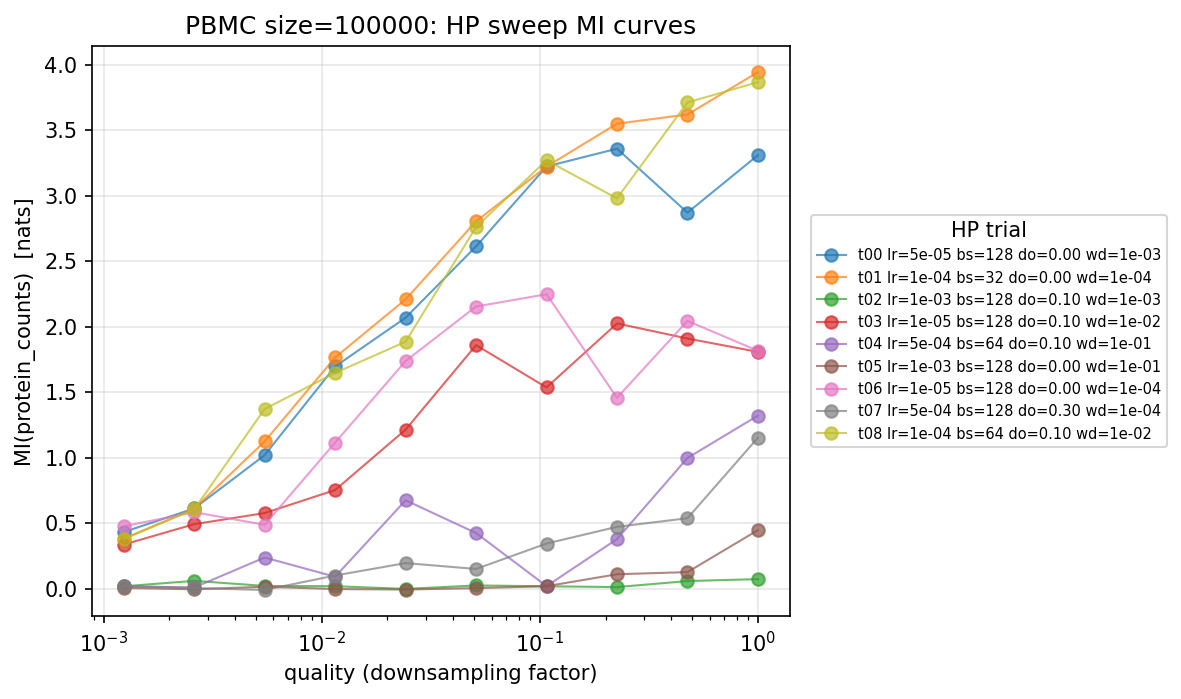
\includegraphics[width=0.85\textwidth,height=0.65\textheight,keepaspectratio]{../final_results/hyperpam_sweep.png}
\caption{STATE hyperparameter sweep on PBMC (100k cells).
Each line is one of the 9 HP configurations; x-axis is quality (log scale),
y-axis is MI on \texttt{protein\_counts} (nats).}
\label{fig:hparam_sweep}
\end{figure}
\clearpage

%% ============================================================
\section{MI Estimator Robustness: KSG vs.\ LMI}

As an estimator-independent cross-check, MI was recomputed using the
KSG $k$-nearest-neighbour estimator ($k{=}3$, base-2 logarithm, values
in bits) on the raw 256-dimensional SCVI embeddings for the shendure
dataset.
KSG operates directly in the original embedding space without any learned
projection or dimensionality reduction, making its assumptions entirely
orthogonal to those of LMI.
The \texttt{author\_day} signal was one-hot encoded via
\texttt{pd.get\_dummies}.
In a second analysis step, the saved KSG and LMI values were loaded
together and compared: a scatter of KSG (bits) vs.\ LMI
(bits, converted from nats) across all 100 (size, quality) combinations
was produced with a linear fit and Pearson/Spearman correlation statistics.
The final CSV and figure saved to \texttt{final\_results} contain only the
KSG values (column \texttt{mi\_bits}), showing KSG MI in bits as a function
of quality with one curve per dataset size; the KSG--LMI correlation
scatter is available in the analysis notebook but not saved here.

\medskip
\noindent\textbf{Data:} \path{analysis/final_results/ksg_vs_quality_shendure_SCVI.csv}

\begin{figure}[H]
\centering
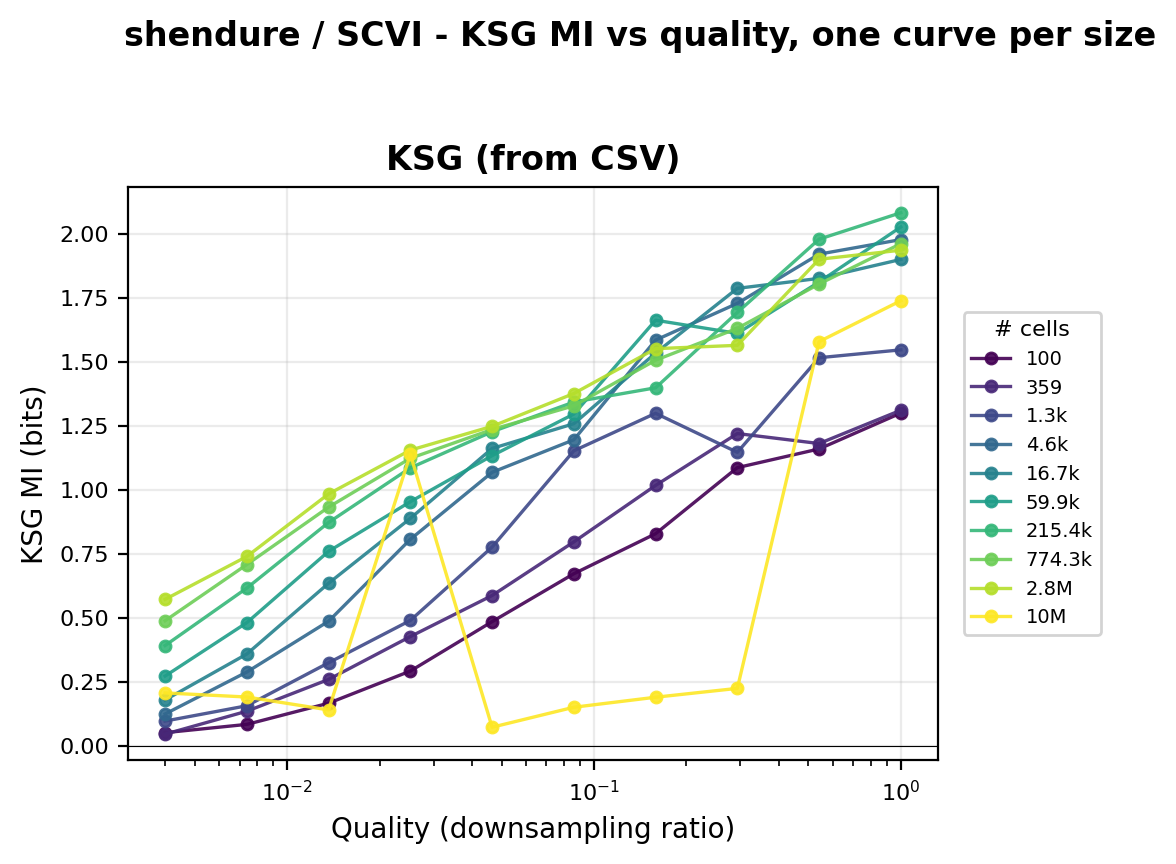
\includegraphics[width=0.85\textwidth,height=0.65\textheight,keepaspectratio]{../final_results/ksg_vs_quality_shendure_SCVI.png}
\caption{KSG MI (bits) for SCVI on shendure vs.\ measurement quality (log
scale), one curve per dataset size.
The KSG--LMI correlation scatter with fit statistics is in the analysis
notebook.}
\label{fig:ksg_vs_lmi}
\end{figure}
\clearpage

%% ============================================================
\section{Linear Probe Scaling Curves}

Supervised probes were trained on top of frozen embeddings to assess
downstream-task performance independently of MI.
The prediction target and probe type differ by dataset:

\begin{itemize}
  \item \textbf{PBMC} --- Ridge regression ($\alpha{=}1.0$) predicting
    surface \texttt{protein\_counts} (multi-output); metrics: mean $R^2$,
    MSE, and MAE across protein channels.
  \item \textbf{MERFISH} --- Ridge regression ($\alpha{=}1.0$) predicting
    the embedding of each cell's nearest-neighbour in gene-expression
    space (\texttt{ng\_idx}); metrics: mean $R^2$, MSE, MAE.
  \item \textbf{larry} --- Lineage prediction via Ridge regression
    ($\alpha{=}1.0$): embeddings of early time-point cells (days 2 and 4)
    are used to predict the embedding of the matched late time-point cell
    (day 6) sharing the same clone barcode.
    Clone-matched pairs are sampled once per clone; clones absent from
    either time point are excluded.
    Metrics: mean $R^2$, MSE, MAE across embedding dimensions.
  \item \textbf{shendure} --- Multi-class \texttt{author\_day}
    classification using a $k$-NN probe ($k{=}5$) and a multinomial
    logistic regression (L-BFGS solver, max iterations 2\,000);
    metrics: accuracy and macro-averaged F1.
\end{itemize}

In all cases the data were split 70/30 (train/test) with seed 42, and
embeddings were subsampled to at most 100\,000 rows where necessary.
All (algorithm, dataset, cell-count, quality) combinations were evaluated
in parallel using 8 workers and assembled into a single long-format table.
Scaling curves were plotted on log--log axes with one curve per algorithm,
as a function of both quality and cell count, with datasets in separate
panels.

\medskip
\noindent\textbf{Data:} \path{analysis/final_results/linear_probe_scaling.csv}

\begin{figure}[H]
\centering
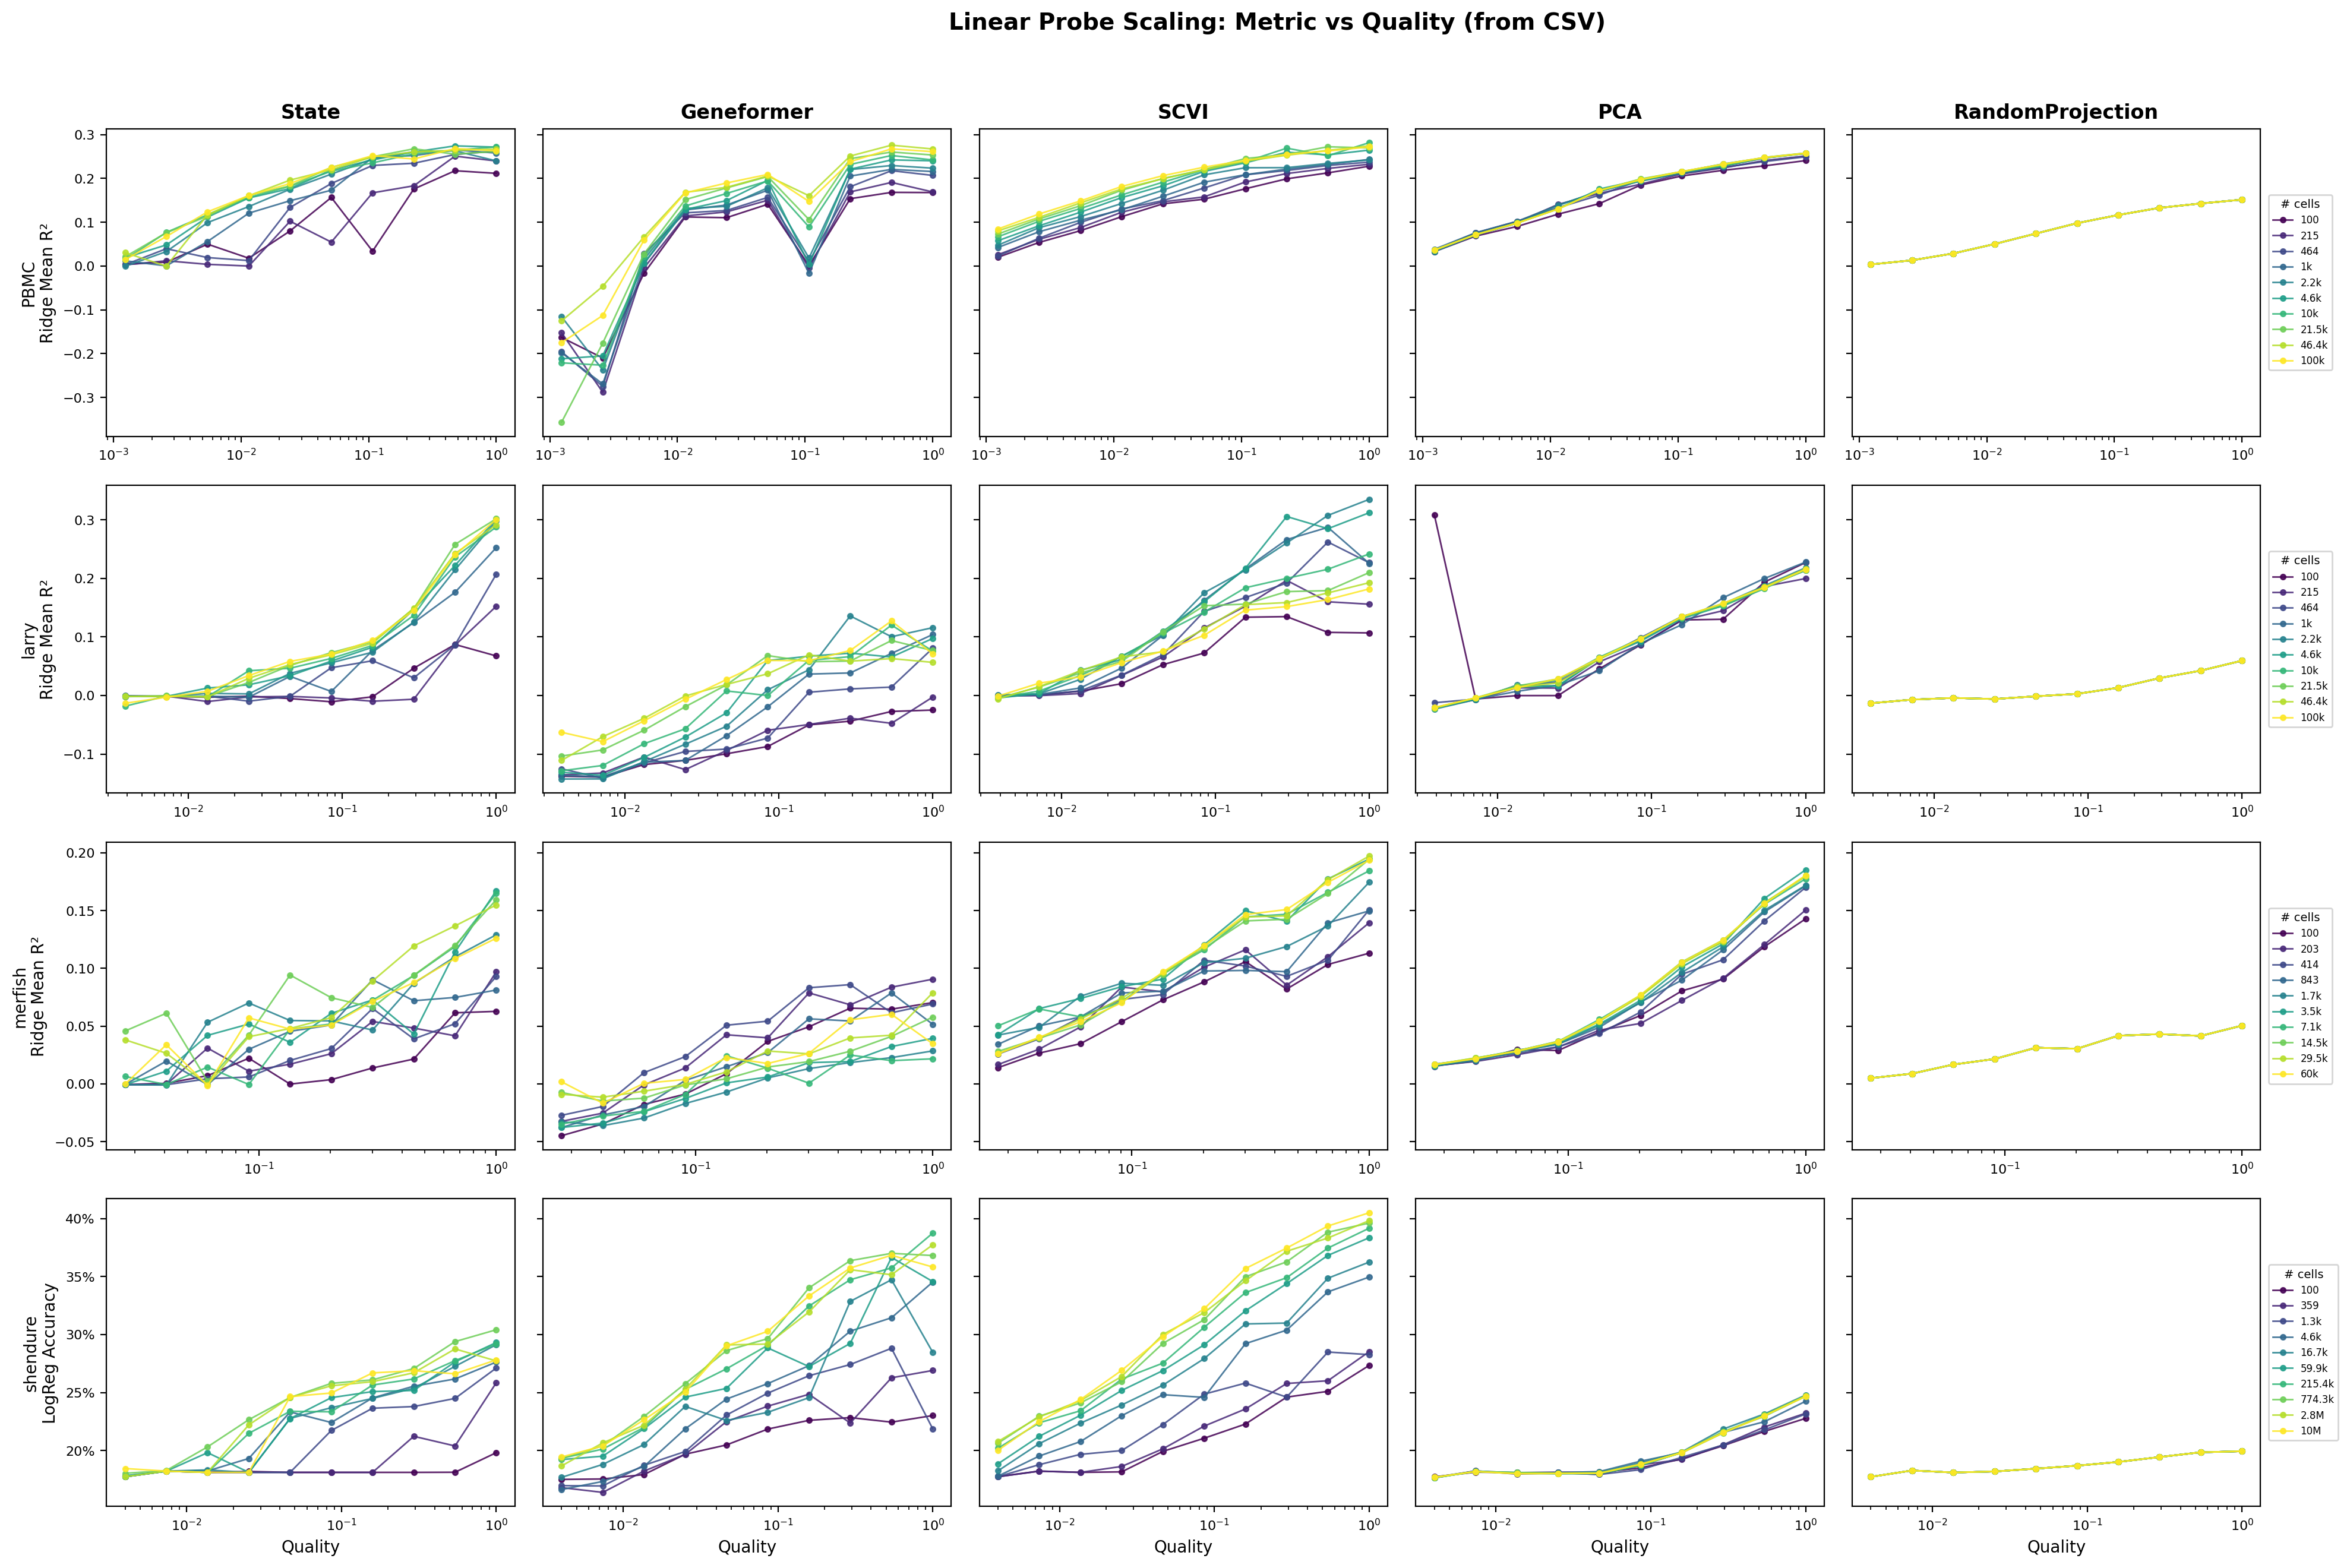
\includegraphics[width=\textwidth,height=0.65\textheight,keepaspectratio]{../final_results/linear_probe_scaling.png}
\caption{Linear probe $R^2$ scaling curves for all algorithms,
plotted against quality and cell count.}
\label{fig:linear_probe}
\end{figure}
\clearpage

%% ============================================================
\section{Learning Trajectory: MI at Each Training Checkpoint}

To study how MI evolves during Geneformer training on the shendure
dataset, LMI was evaluated at 20 evenly-spaced checkpoints for each
(size, quality) combination in the $10 \times 10$ grid.
The checkpoints were identified by scanning the saved
\path{checkpoint-*/} directories and selecting those whose step
indices are evenly spaced between the first and last available
checkpoint.
LMI was computed with \texttt{latentmi} using a fixed random seed
of 42, a maximum of 300 training epochs, and an inference batch size
of 50.
The signal used was \texttt{author\_day}, one-hot encoded.
The evaluation was run across 8 GPUs.
The resulting per-checkpoint MI values were plotted as a function of
training step, with one panel per dataset size and one curve per
quality level within each panel.

\medskip
\noindent\textbf{Data:}
\path{analysis/final_results/shendure_geneformer_checkpoint_mi.csv}

\begin{figure}[H]
\centering
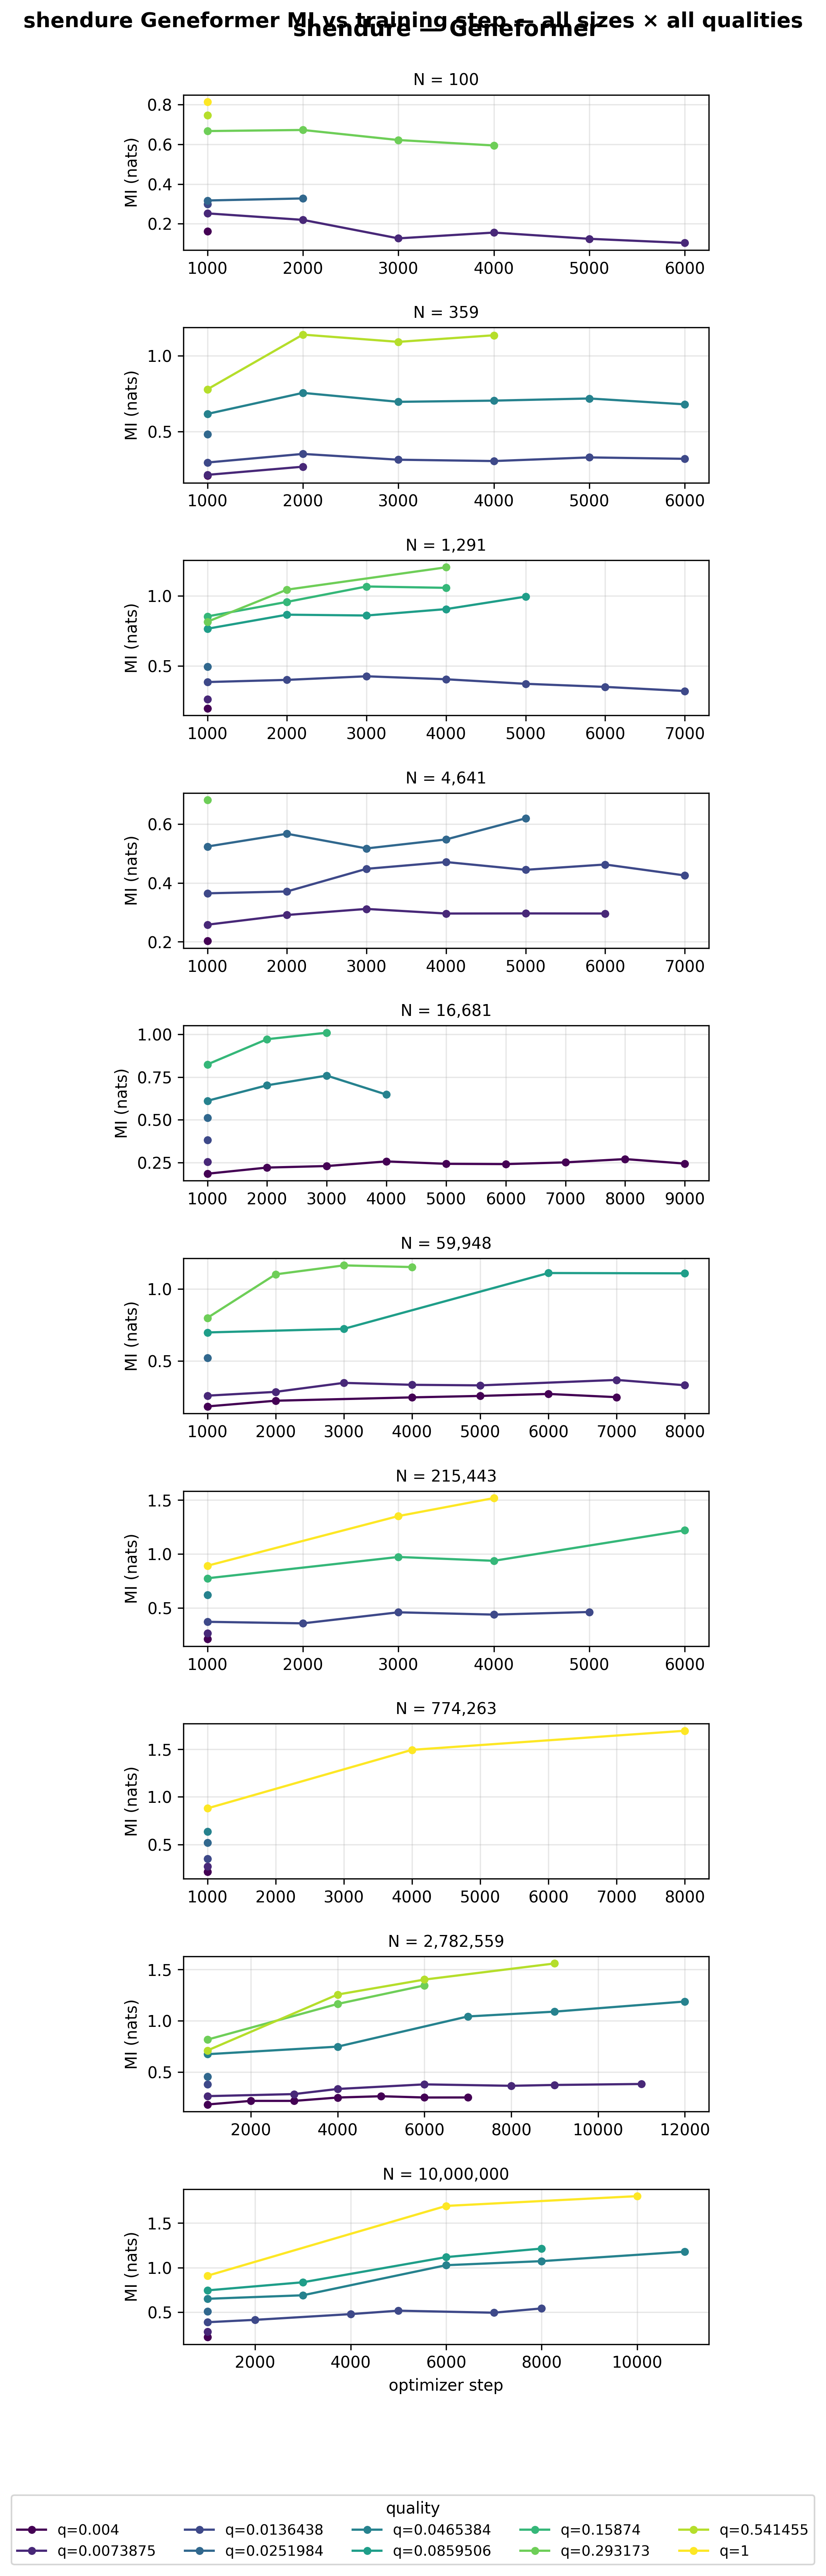
\includegraphics[width=\textwidth,height=0.55\textheight,keepaspectratio]{../final_results/shendure_geneformer_checkpoint_mi.png}
\caption{MI vs.\ training step for Geneformer on shendure.
Panels correspond to dataset sizes; colours indicate quality levels.}
\label{fig:ckpt_mi}
\end{figure}
\clearpage

%% ============================================================
\section{Fine-Tuned Large Pretrained STATE}

The publicly available SE-100M pretrained STATE model
(\path{arcinstitute/SE-100M} on HuggingFace) was fine-tuned on
the full PBMC $10 \times 10$ grid.
The pretrained weights were loaded and the optimiser state was stripped
before fine-tuning began.
Fine-tuning ran for 3 epochs using AdamW.
The peak learning rate was scaled with dataset size:
\begin{equation*}
  \text{lr} = 10^{-6} \times \max\!\left(0.3,\;
    \sqrt{\min\!\left(1,\, \frac{N}{10{,}000}\right)}\right),
\end{equation*}
which gives a floor of $3 \times 10^{-7}$ for the smallest datasets
and caps at $1 \times 10^{-6}$ for all sizes at or above 10\,000 cells.
This is well below the $5 \times 10^{-4}$ used for training from
scratch, to avoid overwriting the pretrained representations.
The per-device batch size was 64 with gradient accumulation over
16 steps, giving an effective batch size of 1\,024.
Dropout was 0.15 for cell counts $\geq$10\,000 and 0.2 for smaller
sizes; weight decay was 0.01 for sizes $\geq$10\,000 and 0.05 otherwise.
Early stopping was disabled; training ran for the full 3 epochs.
Validation loss was recorded every 1\,000 steps (50 batches per check).
After fine-tuning, per-cell embeddings were extracted and LMI was
computed identically to all other experiments on the
\texttt{celltype.l3} and \texttt{protein\_counts} signals.
The resulting MI values were plotted alongside the from-scratch STATE
results and all other algorithm baselines as noise-scaling curves on
a log--log scale.

\medskip
\noindent\textbf{Data:}
\path{analysis/final_results/finetune_se_100m_state_pbmc_noise_scaling.csv}

\begin{figure}[H]
\centering
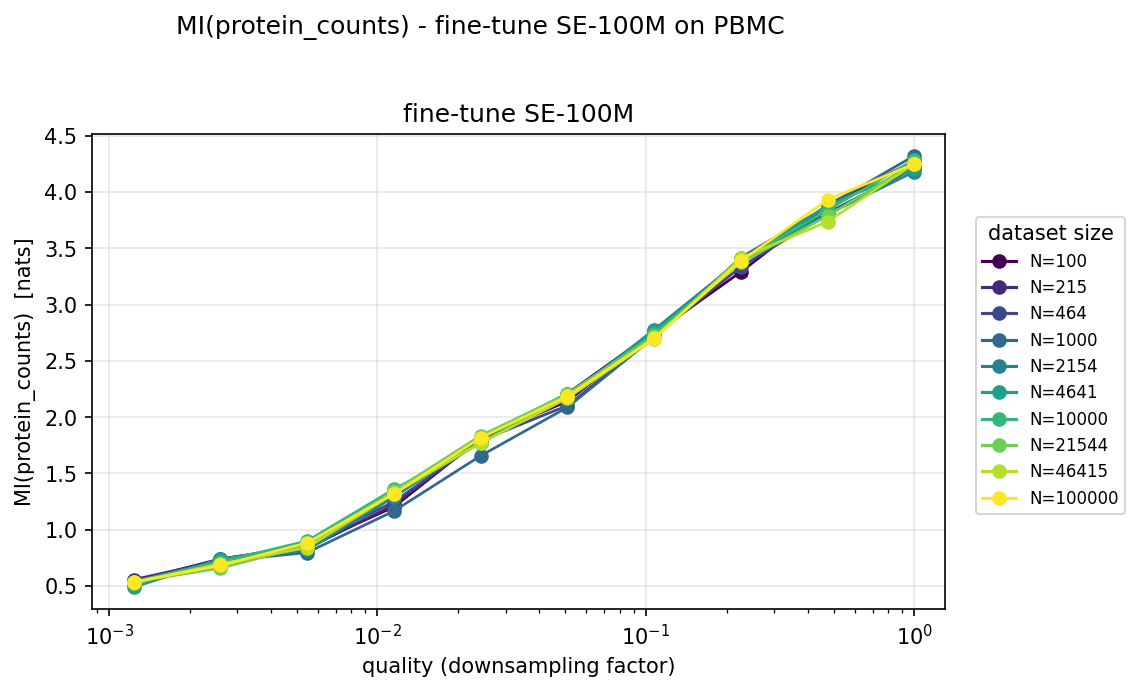
\includegraphics[width=0.85\textwidth,height=0.65\textheight,keepaspectratio]{../final_results/finetune_se_100m_state_pbmc_noise_scaling.png}
\caption{Noise-scaling curves for PBMC: fine-tuned SE-100M STATE
vs.\ from-scratch STATE and other baselines.}
\label{fig:finetune_state}
\end{figure}

\end{document}
